\documentclass{bmstu}

\bibliography{biblio}
\lstset{ %
	basicstyle=\small\sffamily, % размер и начертание шрифта для подсветки кода
	numbers=left,               % где поставить нумерацию строк (слева\справа)
	numberstyle=\tiny,           % размер шрифта для номеров строк
	stepnumber=1,                   % размер шага между двумя номерами строк
	numbersep=5pt,                % как далеко отстоят номера строк от подсвечиваемого кода
	showspaces=false,            % показывать или нет пробелы специальными отступами
	xleftmargin=10pt,
	showstringspaces=false,      % показывать или нет пробелы в строках
	showtabs=false,             % показывать или нет табуляцию в строках
	frame=single,              % рисовать рамку вокруг кода
	tabsize=2,                 % размер табуляции по умолчанию равен 2 пробелам
	captionpos=t,              % позиция заголовка вверху [t] или внизу [b] 
	breaklines=true,           % автоматически переносить строки (да\нет)
	breakatwhitespace=false, % переносить строки только если есть пробел
	escapeinside={\#*}{*)}   % если нужно добавить комментарии в коде
}

\usepackage[scientific-notation=false]{siunitx}
\usepackage{pdfpages}
\newcommand{\specialcell}[2][c]{%
	\begin{tabular}[#1]{@{}c@{}}#2\end{tabular}}
\begin{document}

\makereporttitle{Информатика и системы управления}{Программное обеспечение ЭВМ и информационные технологии}{лабораторной работе №1}{Защита информации}{Моделирование шифровальной машины <<Энигма>>}{}{ИУ7-72Б}{Е.~О.~Карпова}{И.~С.~Чиж}

\maketableofcontents

%\begin{definitions}
	\definition{База данных}{совокупность данных из определённой предметной области, организованных по определённым правилам, предусматривающим общие принципы описания, хранения и манипулирования данными, независимая от прикладных программ~\cite{bib41}.}
	\definition{Модель данных}{абстрактная модель, определяющая совокупность правил создания и использования данных, описывающая способ представления данных, доступ к ним и связи между ними в той или иной области~\cite{bib13}.}
	\definition{Система управления базами данных}{это совокупность программ и языковых средств, предназначенных для управления данными в базе данных, ведения базы данных и обеспечения взаимодействия её с прикладными программами~\cite{bib41}.}
	\definition{Брокер сообщений}{программное обеспечение, которое позволяет приложениям, системам и службам взаимодействовать друг с другом и обмениваться информацией~\cite{bib43}.}
	\definition{Топик}{логическая категория сообщений~\cite{bib44}.}
	\definition{Партиция}{физическое хранилище сообщений в кластере Kafka~\cite{bib44}.}
	\definition{Движок таблицы}{тип таблицы, определяющий способ хранения и получения данных, поддерживаемые виды запросов и иные параметры работы с данными~\cite{bib45}.}
	\definition{Аутентификация}{это проверка соответствия субъекта и того, за кого он пытается себя выдать с помощью некой уникальной информации~\cite{bib42}.}
\end{definitions}
%\begin{abbreviations}
	\definition{БД}{База Данных.}
	\definition{СУБД}{Система Управления Базами Данных.}
	\definition{ACID}{Atomicity, Consistency, Isolation, Durability.}
	\definition{API}{Application Programming Interface.}
	\definition{MVVM}{Model-View-ViewModel.}
	\definition{JWT}{JSON Web Token.}
	\definition{АКИТ}{Ассоциация Компаний Интернет-Торговли.}
	\definition{HTML}{HyperText Markup Manguage.}
	\definition{JSON}{JavaScript Object Notation.}
	\definition{SQL}{Structured Query Language.}
	\definition{ПО}{Программное Обеспечение.}
	\definition{SMTP}{Simple Mail Transfer Protocol.}
	\definition{SPA}{Single Page Application.}
\end{abbreviations}

\chapter*{ВВЕДЕНИЕ}
\addcontentsline{toc}{chapter}{ВВЕДЕНИЕ}

Транслятор~---~это программа перевода текста программы с исходного языка на объектный~\cite{bib1}. Если исходный язык является языком программирования высокого уровня, и, если объектный язык~---~язык ассемблера или машинный язык, то транслятор называют \textbf{компилятором}. Трансляция исходной программы в объектную выполняется во время компиляции, а фактическое выполнение объектной программы во время выполнения готовой программы.

Целью данной работы является разработка компилятора языка Lua. Компилятор должен выполнять чтение текстового файла, содержащего код на языке Lua и генерировать на выходе программу, пригодную для запуска.


В ходе работы необходимо решить следующие задачи:
\begin{enumerate}
	\item Проанализировать грамматику языка Lua и выделить ее ключевые составляющие.
	\item Изучить существующие средства для анализа исходных кодов программ, системы для генерации низкоуровневого кода, запуск которого возможен на большинстве из используемых платформ и операционных систем.
	\item Разработать прототип компилятора на языке Go, выполняющий синтаксический анализ исходного текста программы и построение абстрактного синтаксического дерева.
	\item Провести преобразование абстрактного синтаксического дерева в IR с использованием LLVM.
\end{enumerate}
\chapter{Аналитический раздел}

%\par В этом разделе будет проведён анализ предментой области и обзор существующих решений, обоснована актуальность решаемой продуктом задачи. Также, будет формализована задача, пользовательские сценарии, данные и выбрана модель данных, тип базы данных и тип системы управления базой данных. 

\section{Устройство компилятора}

Процесс компиляции состоит из следующих этапов~\cite{compilers}.
\begin{enumerate}
	\item Лексический анализ. 
	\item Синтаксический анализ. 
	\item Семантический анализ.
	\item Генерация кода на языке целевой платформы.
\end{enumerate}

\section{Лексический анализатор}

Лексический анализ~---~распознавание базовых элементов языка, перевод исходной программы в поток лексем и передача токенов, образуемых этими лексемами, последующим стадиям компиляции.


Основные функции лексического анализатора:
\begin{itemize}
	\item удаление пробелов и комментариев, обнаружение лексических ошибок;
	\item сборка последовательности цифр, формирующих константу;
	\item распознавание идентификаторов и ключевых слов.
\end{itemize}

\begin{table}[h!]
	\centering
	\begin{tabular}{p{1\linewidth}}
	  \centering
	  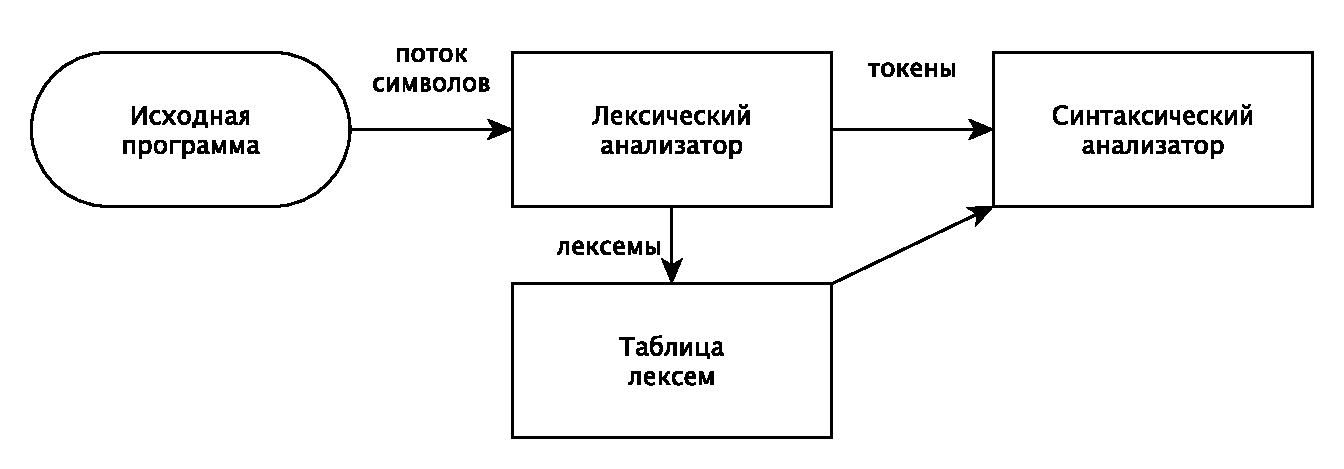
\includegraphics[width=0.8\linewidth]{./images/lexer.pdf}
	  \captionof{figure}{Лексический анализатор}
	  \label{img:lexer}
	\end{tabular}
  \end{table}

\section{Синтаксический анализатор}

Вторая фаза компилятора~---~синтаксический анализ или разбор. Анализатор использует первые компоненты токенов, полученных при лексическом анализе, для создания древовидного промежуточного представления, которое описывает грамматическую структуру потока токенов. 
Типичным представлением является синтаксическое дерево.

Полученная грамматическая структура используется в последующих этапах компиляции для анализа исходной программы и генерации кода для целевой платформы.
Синтаксический анализ выявляет синтаксические ошибки, относящиеся к нарушению структуры программы.

\begin{table}[h!]
	\centering
	\begin{tabular}{p{1\linewidth}}
	  \centering
	  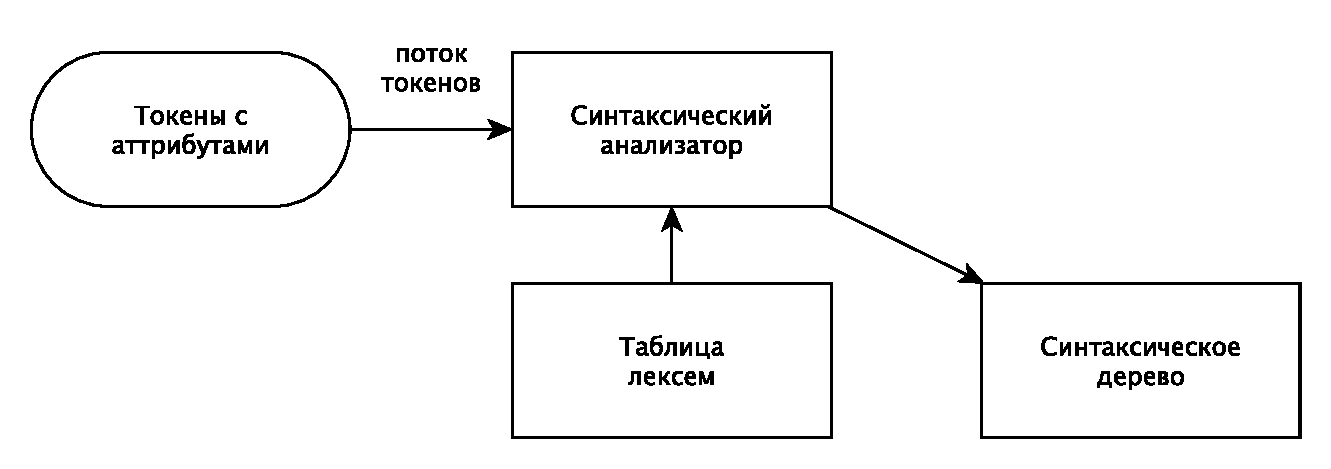
\includegraphics[width=0.8\linewidth]{./images/syntax.pdf}
	  \captionof{figure}{Синтаксический анализатор}
	  \label{img:syntax}
	\end{tabular}
  \end{table}

\section{Семантический анализатор}

Семантический анализатор использует синтаксическое дерево и информацию из таблицы символов для проверки исходной программы на семантическую согласованность с определением языка. Он также собирает информацию о типах и сохраняет все в синтаксическом дереве или в таблице символов для последующего использования в процессе генерации промежуточного кода.

Важной частью семантического анализа является проверка типов, когда компилятор проверяет, имеет ли каждый оператор операнды соответствующего типа.

Как правило, семантический анализатор разделяется на ряд более мелких, каждый из которых предназначен для конкретной конструкции. Соответствующий семантический анализатор вызывается синтаксическим анализатором как только он распознает синтаксическую единицу, требующую обработки.

\begin{table}[h!]
	\centering
	\begin{tabular}{p{1\linewidth}}
	  \centering
	  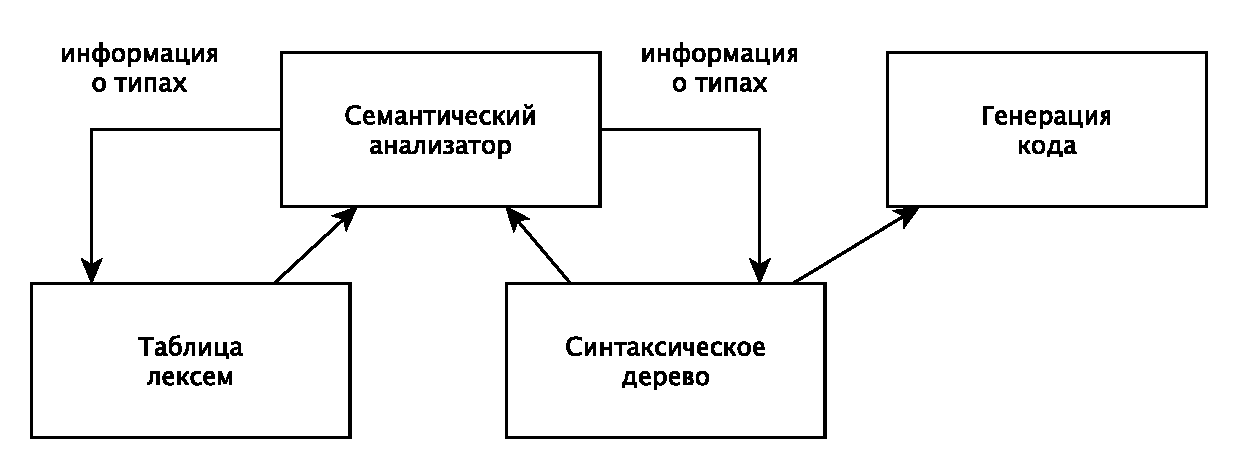
\includegraphics[width=0.8\linewidth]{./images/sem.pdf}
	  \captionof{figure}{Семантический анализатор}
	  \label{img:sem}
	\end{tabular}
  \end{table}

\section{Генерация кода}

\subsection{Генерация промежуточного кода}

В процессе трансляции исходной программы в целевой код компилятор может создавать одно или несколько промежуточных представлений различного вида.
Синтаксические деревья являются видом промежуточного представления. Обычно они используются в процессе синтаксического и семантического анализа.

После синтаксического и семантического анализа исходной программы многие компиляторы генерируют явное низкоуровневое или машинное промежуточное представление исходной программы, которое можно рассматривать как программу для абстрактной вычислительной машины. 
Такое промежуточное представление должно обладать двумя важными свойствами: оно должно легко генерироваться и легко транслироваться в целевой машинный язык.

\subsection{Оптимизация}

Фаза машинно-независимой оптимизации кода пытается улучшить промежуточный код, чтобы затем получить более качественный целевой код. Например, более быстрый код, короткий код, или код, использующий меньшее количество ресурсов. 

\subsection{Генерация кода на целевом языке}

Генератор кода получает в качестве входных данных промежуточное представление исходной программы и отображает его в целевой язык. 
Если целевой язык представляет собой машинный код, для каждой переменной, используемой программой, выбираются соответствующие регистры или ячейки памяти. 
Затем промежуточные команды транслируются в последовательности машинных команд, выполняющих те же действия.

\section{Таблица символов}

Важная функция компилятора состоит в том, чтобы записывать имена переменных в исходной программе и накапливать информацию о разных атрибутах каждого имени. 
Эти атрибуты могут предоставлять информацию о выделенной памяти для данного имени, его типе, области видимости и, в случае имен процедур, такие сведения, как количество и типы их аргументов, метод передачи каждого аргумента, а также возвращаемый тип.
Таблица символов представляет собой структуру данных, содержащую записи для каждого имени переменной, с полями для атрибутов имени. 

\section{Синтаксическое дерево}

Синтаксическое дерево~---~дерево, в котором каждый внутренний узел представляет операцию, а дочерние узлы~---~аргументы этой операции.
Порядок операций в дереве согласуется с обычными правилами, например, умножение имеет более высокий приоритет, чем сложение, и должно быть выполнено до сложения.

\begin{table}[h!]
	\centering
	\begin{tabular}{p{1\linewidth}}
	  \centering
	  \includegraphics[width=1\linewidth]{./images/tree.png}
	  \captionof{figure}{Пример синтаксического дерева}
	  \label{img:tree}
	\end{tabular}
  \end{table}

\section{Генераторы лексических анализаторов}

Существует множество генераторов, наиболее популярные из них~---~Lex, Flex и ANTLR4.

Lex~---~стандартный инструмент для получения лексических анализаторов в операционных системах Unix~\cite{lesk1975lex}. 
В результате обработки входного потока получается исходный файл на языке C. 
Lex-файл разделяется на три блока: блок определений, правил и кода на C. 

Flex заменяет Lex в системах на базе пакетов GNU и имеет аналогичную функциональность~\cite{sampath2007test}.

ANTLR (ANother Tool for Language Recognition)~---~генератор лексических и синтаксических анализаторов, позволяет создавать анализаторы на таких языках, как: Java, C\#, Go, C++ и других~\cite{parr2004s}.

ANTLR генерирует классы нисходящего рекурсивного синтаксического анализатора, на основе правил, заданных грамматикой. 

Он также позволяет строить и обходить деревья синтаксического анализа с использованием паттернов посетитель или слушатель. 
Благодаря своей эффективности и простоте использования, ANTLR является одним из наиболее предпочтительных генераторов анализаторов при создании кода синтаксического анализатора. 
В текущей работе было решено использовать этот инструмент.

\section{Генераторы синтаксических анализаторов}

Для создания синтаксических анализаторов используются такие инструменты, как Yacc/Bison, Coco/R и описанный ранее ANTLR.

Yacc~---~стандартный генератор синтаксических парсеров в Unix системах, Bison~---~аналогичный ему генератор для GNU систем~\cite{yacc}.

Coco/R~---~генератор лексических и синтаксических анализаторов~\cite{mossenbock2003compilergenerator}. 
Лексические анализаторы работают по принципу конечных автоматов, а синтаксические используют рекурсивный спуск. 
Поддерживаются такие языки программирования, как C\+\+, C\#, Java и другие.

Yacc принимает на вход контекстно-свободную грамматику и использует LALR-разбор (LR-разбор с предпросмотром). 
Канонические LR-анализаторы имеют незначительно большую распознавающую способность, чем LALR-анализаторы, однако требуют намного больше памяти для таблиц, поэтому их используют очень редко.

ANTLR и Coco/R принимают на вход контекстно-свободную грамматику, ANTLR использует LL(*)-разбор, а также умеет работать с левой рекурсией, чего не могут
обычные LL-анализаторы, Coco/R использует LL(1)-разбор.

LL-анализатор называется LL(k)-анализатором, если данный анализатор использует предпросмотр на k токенов при разборе входного потока.

LR-анализаторы, в отличие от LL-анализаторов, строящих левосторонний вывод, производят наиболее правую продукцию контекстно-свободной грамматики.
LR-анализ может применяться к большему количеству языков, чем LL-анализ, а также лучше в части сообщения об ошибках, 
то есть он определяет синтаксические ошибки там, где вход не соответствует грамматике, как можно раньше. 
В отличие от этого, LL(k) анализаторы могут задерживать определение ошибки до другой ветки грамматики из-за отката, 
часто затрудняя определение места ошибки в местах общих длинных префиксов. Однако, в большинстве случаев LL-разбор работает быстрее LR-разбора,
а LR-анализаторы и построение их таблиц сложнее в реализации.

\section{LLVM}

LLVM (Low Level Virtual Machine)~---~проект программной инфраструктуры для создания компиляторов и сопутствующих им утилит~\cite{sarda2015llvm}. 
В его основе лежит платформонезависимая система кодирования машинных инструкций~---~байткод LLVM IR. 
LLVM может создавать байткод для множества платформ, включая ARM, x86, x86-64, GPU от AMD и Nvidia и другие. 
Для компиляции LLVM IR в код платформы используется clang. 
В состав LLVM входит также интерпретатор LLVM IR, способный исполнять код без компиляции в код платформы.

LLVM поддерживает целые числа произвольной разрядности, числа с плавающей точкой, массивы, структуры и функции. 
Большинство инструкций в LLVM принимает два аргумента и возвращает одно значение.
Значения в LLVM определяются текстовым идентификатором. 
Тип операндов всегда указывается явно и однозначно определяет тип результата. 
Операнды арифметических инструкций должны иметь одинаковый тип, но сами инструкции «перегружены» для любых числовых типов и векторов.
LLVM IR строго типизирован, поэтому существуют операции приведения типов, которые явно кодируются специальными инструкциями. 
Кроме того, существуют инструкции преобразования между целыми числами и указателями, а также универсальная инструкция для приведения типов bitcast.
Значения в памяти адресуются типизированными указателями. 
Обратиться к ней можно с помощью двух инструкций: load и store. Инструкция alloca выделяет память на стеке. 
Она автоматически освобождается при выходе из функции.
Для вычисления адресов элементов массивов и структур с правильной типизацией используется инструкция getelementptr. 
Она только вычисляет адрес без обращения к памяти, принимает произвольное количество индексов и может разыменовывать структуры любой вложенности.

\section{Вывод}

В данном разделе приведён обзор основных фаз компиляции, описана каждая из них. 
Также был выбран генератор лексического и синтаксического анализаторов~---~ANTLR и LLVM в качестве генератора машинного кода.


















 

\chapter{Конструкторский раздел}

%В данном разделе будет проведена формализация сущностей проектируемой системы, описаны используемые домены, ролевая модель и реализуемая табличная функция.

\section{Формализация сущностей системы}
Обозначения в таблицах: PK~---~первичный ключ, FK~---~внешний ключ, U~---~уникальное значение, NN~---~поле не может принимать неопределённое значение, I~---~целочисленный тип, B~---~логический тип, DT~---~тип временной отметки, SP~---~тип временного интервала, S~---~символьный тип, L~---~логический тип, J~---~JSON, ID~---~тип идентификатора.

\paragraph{Таблица Client}\mbox{}

В таблице Client содержится информация о клиентах основной системы. Описание полей таблицы Client представлено в таблице~\ref{table:client}.

\begin{table}[H]
	\begin{center}
		\caption{\label{table:client} Описание полей таблицы Client}
		\begin{tabular}{|l|c|c|c|c|c|l|}
			\hline
			{\specialcell{\\Название}} & \multicolumn{6}{c|}{\specialcell{Характеристики}}\\ \cline{2-7}
			&{PK}&{FK}&{U}&{NN}&{Тип}&{Значение}\\ \hline
			
			id & $+$ & $-$ & $+$ & $+$ & ID & {\specialcell{Идентификатор клиента}}\\ \hline
			name & $-$ & $-$ & $-$ & $+$ & S & {\specialcell{Имя клиента}}\\ \hline
			surname & $-$ & $-$ & $-$ & $+$ & S & {\specialcell{Фамилия клиента}}\\ \hline
			patronymic & $-$ & $-$ & $-$ & $-$ & S & {\specialcell{Отчество клиента}}\\ \hline
			birthDate & $-$ & $-$ & $-$ & $+$ & DT & {\specialcell{Дата рождения}}\\ \hline
			registrationDate & $-$ & $-$ & $-$ & $+$ & DT & {\specialcell{Дата регистрации}}\\ \hline
			gender & $-$ & $-$ & $-$ & $+$ & S & {\specialcell{Пол клиента}}\\ \hline
			email & $-$ & $-$ & $+$ & $+$ & S & {\specialcell{Адрес электронной почты}}\\ \hline
			data & $-$ & $-$ & $-$ & $-$ & J & {\specialcell{Дополнительная информация}}\\ \hline
			
		\end{tabular}
	\end{center}
\end{table}

\newpage

\paragraph{Таблица User}\mbox{}

В таблице User содержится информация о пользователей системы рассылки. Описание полей таблицы User представлено в таблице~\ref{table:user}.

\begin{table}[H]
	\begin{center}
		\caption{\label{table:user} Описание полей таблицы User}
		\begin{tabular}{|l|c|c|c|c|c|l|}
			\hline
			{\specialcell{\\Название}} & \multicolumn{6}{c|}{\specialcell{Характеристики}}\\ \cline{2-7}
			&{PK}&{FK}&{U}&{NN}&{Тип}&{Значение}\\ \hline
			
			id & $+$ & $-$ & $+$ & $+$ & ID & {\specialcell{Идентификатор пользователя}}\\ \hline
			login & $-$ & $-$ & $+$ & $+$ & S & {\specialcell{Логин пользователя}}\\ \hline
			password & $-$ & $-$ & $-$ & $+$ & S & {\specialcell{Пароль пользователя}}\\ \hline
			isAdmin & $-$ & $-$ & $-$ & $+$ & B & {\specialcell{Уровень доступа в системе}}\\ \hline
			
		\end{tabular}
	\end{center}
\end{table}

\paragraph{Таблица Event}\mbox{}

В таблице Event содержится информация о событиях основной системы. Описание полей таблицы Event представлено в таблице~\ref{table:event}.

\begin{table}[H]
	\begin{center}
		\caption{\label{table:event} Описание полей таблицы Event}
		\begin{tabular}{|l|c|c|c|c|c|l|}
			\hline
			{\specialcell{\\Название}} & \multicolumn{6}{c|}{\specialcell{Характеристики}}\\ \cline{2-7}
			&{PK}&{FK}&{U}&{NN}&{Тип}&{Значение}\\ \hline
			
			id & $+$ & $-$ & $+$ & $+$ & ID & {\specialcell{Идентификатор события}}\\ \hline
			alias & $-$ & $-$ & $-$ & $+$ & S & {\specialcell{Идентификатор типа события}}\\ \hline
			clientID & $-$ & $+$ & $-$ & $-$ & ID & {\specialcell{Идентификатор инициатора}}\\ \hline
			eventTime & $-$ & $-$ & $-$ & $+$ & DT & {\specialcell{Время события}}\\ \hline
			
		\end{tabular}
	\end{center}
\end{table}

\paragraph{Таблица EventType}\mbox{}

В таблице EventType содержится информация о типах событий основной системы. Описание полей таблицы EventType представлено в таблице~\ref{table:eventtype}.

\begin{table}[H]
	\begin{center}
		\caption{\label{table:eventtype} Описание полей таблицы EventType}
		\begin{tabular}{|l|c|c|c|c|c|l|}
			\hline
			{\specialcell{\\Название}} & \multicolumn{6}{c|}{\specialcell{Характеристики}}\\ \cline{2-7}
			&{PK}&{FK}&{U}&{NN}&{Тип}&{Значение}\\ \hline
			
			id & $+$ & $-$ & $+$ & $+$ & ID & {\specialcell{Идентификатор события}}\\ \hline
			name & $-$ & $-$ & $-$ & $+$ & S & {\specialcell{Название события}}\\ \hline
			alias & $-$ & $-$ & $+$ & $+$ & S & {\specialcell{Псевдоним события}}\\ \hline
			
		\end{tabular}
	\end{center}
\end{table}

\paragraph{Таблица Ad}\mbox{}

В таблице Ad содержится информация о рекламных записях для рассылки. Описание полей таблицы Ad представлено в таблице~\ref{table:ad}.

\begin{table}[H]
	\begin{center}
		\caption{\label{table:ad} Описание полей таблицы Ad}
		\begin{tabular}{|l|c|c|c|c|c|l|}
			\hline
			{\specialcell{\\Название}} & \multicolumn{6}{c|}{\specialcell{Характеристики}}\\ \cline{2-7}
			&{PK}&{FK}&{U}&{NN}&{Тип}&{Значение}\\ \hline
			
			id & $+$ & $-$ & $+$ & $+$ & ID & {\specialcell{Идентификатор рассылки}}\\ \hline
			content & $-$ & $-$ & $-$ & $+$ & S & {\specialcell{Содержимое записи}}\\ \hline
			filters & $-$ & $-$ & $-$ & $+$ & J & {\specialcell{Фильтры рассылки}}\\ \hline
			createTime & $-$ & $-$ & $-$ & $+$ & DT & {\specialcell{Время создания}}\\ \hline
			userID & $-$ & $+$ & $-$ & $-$ & ID & {\specialcell{Идентификатор создателя}}\\ \hline
			scheduleID & $-$ & $+$ & $+$ & $+$ & ID & {\specialcell{Идентификатор расписания}}\\ \hline
			
		\end{tabular}
	\end{center}
\end{table}

\newpage

\paragraph{Таблица Schedule}\mbox{}

В таблице Schedule содержится информация о расписаниях для рассылок. Описание полей таблицы Schedule представлено в таблице~\ref{table:schedule}.

\begin{table}[H]
	\begin{center}
		\caption{\label{table:schedule} Описание полей таблицы Schedule}
		\begin{tabular}{|l|c|c|c|c|c|l|}
			\hline
			{\specialcell{\\Название}} & \multicolumn{6}{c|}{\specialcell{Характеристики}}\\ \cline{2-7}
			&{PK}&{FK}&{U}&{NN}&{Тип}&{Значение}\\ \hline
			
			id & $+$ & $-$ & $+$ & $+$ & ID & {\specialcell{Идентификатор расписания}}\\ \hline
			nextTime & $-$ & $-$ & $-$ & $+$ & DT & {\specialcell{Время следующей рассылки}}\\ \hline
			span & $-$ & $-$ & $-$ & $+$ & SP & {\specialcell{Интервал рассылки}}\\ \hline
			finished & $-$ & $-$ & $-$ & $+$ & B & {\specialcell{Активность рассылки}}\\ \hline
			periodic & $-$ & $-$ & $-$ & $+$ & B & {\specialcell{Периодичность рассылки}}\\ \hline
			
		\end{tabular}
	\end{center}
\end{table}

\section{Домены}
Для контроля валидности данных введены следующие домены:
\begin{enumerate}
	\item etType~---~временная метка с ограничениями: не позже, чем текущий момент времени.
	\item genderType~---~перечисление, имеющее 2 возможных значения: male, female.
	\item bdType~---~временная метка с ограничениями: не позже, чем текущий момент времени и не ранее, чем 01.01.1900 00:00:00.
	\item rdType~---~временная метка с ограничениями: не позже, чем текущий момент времени, не ранее, чем дата рождения.
	\item loginType~---~символьный тип с ограничениями: не менее 5 символов.
	\item aliasType~---~символьный тип с ограничениями: не менее 5 символов.
	\item ctType~---~временная метка с ограничениями: не позже, чем текущий момент времени.
\end{enumerate}

На рисунке~\ref{img:martin} представлена ER-диаграмма сущностей в нотации Мартина.

\begin{table}[h!]
  \centering
  \begin{tabular}{p{1\linewidth}}
    \centering
    \includegraphics[width=1\linewidth]{./images/martin.pdf}
    \captionof{figure}{ER-диаграмма сущностей в нотации Мартина}
    \label{img:martin}
  \end{tabular}
\end{table}

\section{Ролевая модель на уровне базы данных}
На уровне взаимодействия с базой данных представлена следующая ролевая модель:
\begin{enumerate}
	\item Client~---~пользователь основной системы. Обладает правами на: \begin{itemize}
		\item \texttt{INSERT} в таблицу клиентов Client;
		\item \texttt{INSERT} в таблицу событий Events.
		\end{itemize}
	\item Targetologist~---~таргетолог, координирующий рекламную рассылку. Обладает правами на: \begin{itemize}
		\item \texttt{SELECT}, \texttt{INSERT} в таблицу пользователей User;
		\item \texttt{SELECT}, \texttt{INSERT} в таблицу рассылок Ad;
		\item \texttt{SELECT}, \texttt{INSERT} в таблицу типов событий EventType;
		\item \texttt{SELECT}, \texttt{INSERT}, \texttt{UPDATE} в таблицу расписания Schedule;
		\item \texttt{SELECT} в таблицу клиентов Client;
		\item \texttt{SELECT} в таблицу событий Events.
		\end{itemize}
	\item Administrator~---~администратор системы. Обладает правами на: \begin{itemize}
		\item \texttt{SELECT}, \texttt{INSERT}, \texttt{DELETE}, \texttt{UPDATE} в таблицу пользователей User;
		\item \texttt{SELECT}, \texttt{DELETE} в таблицу клиентов Client.
		\end{itemize}
\end{enumerate}

\section{Разработка табличной функции}
Необходимо разработать табличную функцию, реализующую выборку записей, соответствующих записям о рекламной рассылке, которую необходимо отправить в заданный временной интервал. Записи выбираются из таблицы, сформированной объединением таблицы рассылок Ad с таблицей расписания Schedule.

Схема соответствующей табличной функции \texttt{get\_ads\_by\_span} представлена на рисунке~\ref{img:func}.

\newpage

\begin{table}[h!]
  \centering
  \begin{tabular}{p{1\linewidth}}
    \centering
    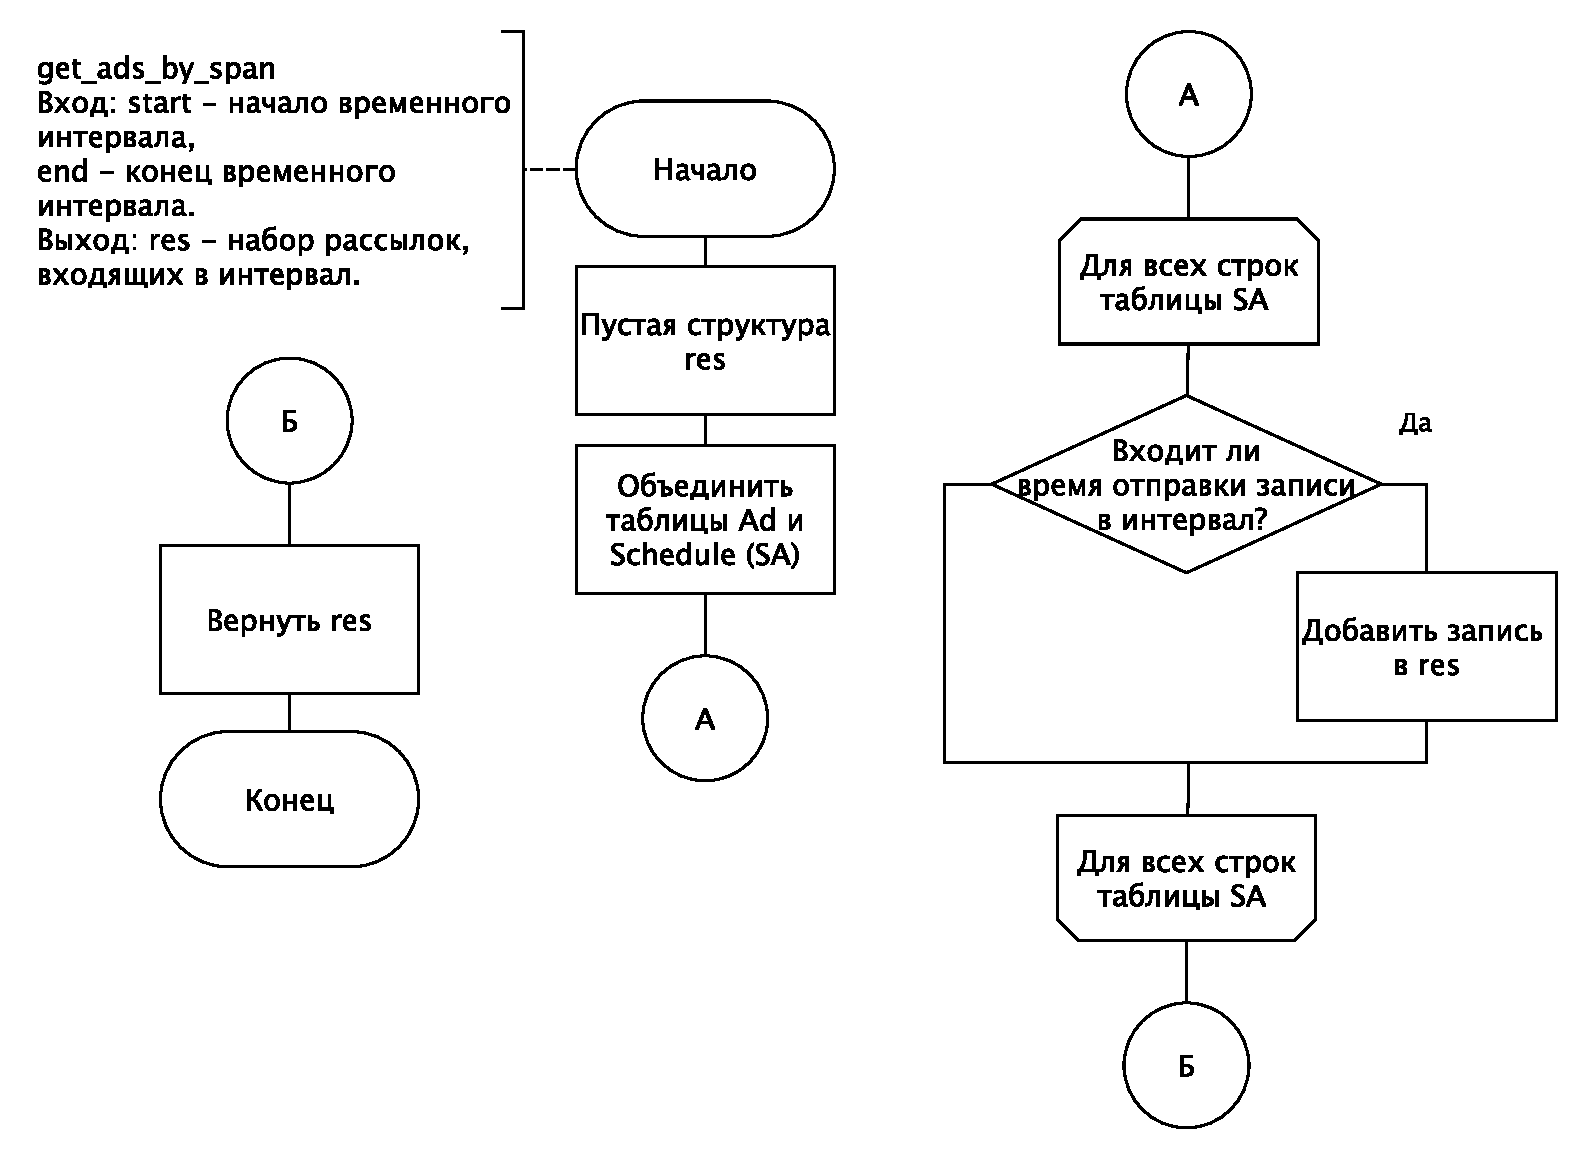
\includegraphics[width=1\linewidth]{./images/func.pdf}
    \captionof{figure}{Схема табличной функции \texttt{get\_ads\_by\_span}}
    \label{img:func}
  \end{tabular}
\end{table}

\section{Вывод}
В данном разделе была проведена формализация сущностей проектируемой системы: на каждую сущность приведена таблица, описывающая её характеристики и необходимые атрибуты. Также, описаны используемые домены, позволяющие поддерживать целостность и непротиворечивость системы, и ролевая модель, определяющая права доступа пользователей к объектам базы данных. Представлена схема алгоритма работы реализуемой табличной функции, осуществляющей выборку записей о рекламной рассылке, которую нужно отправить в заданный интервал времени, реализация которой приведена в листинге Приложения~А.

\chapter{Технологический раздел}

%В данном разделе описан выбор системы управления базой данных, средств разработки серверной и клиентской частей ПО, интерфейсов и представлена общая схема взаимодействия компонентов системы. Также, описаны методы тестирования и обеспечения безопасности данных.

\section{Выбор средств программной реализации}

В качестве языка программирования был выбран язык Go, ввиду следующих причин.
\begin{itemize}
	\item Компилятор, написанный на Go может быть запущен на различных платформах.
	\item Для языка Go существуют библиотеки, позволяющие генерировать код для LLVM.
	\item Выбранный генератор лексических и синтаксических анализаторов ANTLR позволяет генерировать код на Go.
\end{itemize}

\section{Основные компоненты программы}

В результате работы ANTLR были сгенерированы интерфейсы для Visitor и Listener, файлы с данными для интерпретатора ANTLR, файлы с токенами и реализации анализаторов.

На языке Go был реализован интерфейс Visitor, так как, несмотря на большие требования по контролю за обходом дерева, он предоставляет больше гибкости в анализе дерева и позволяет возвращать значения из обработчиков.
Для каждой семантической единицы была прописана собственная логика анализа. 

\includelistingpretty{semantic}{}{Пример реализации посещения для оператора логического "или"}

Примеры программ на Lua и соответствующий им результат работы компилятора на LLVM IR представлены в Приложении~Б.

Язык Lua имеет обладает специфическими особенностями, что вызвало необходимость в реализации дополнительного функционала. Далее представлено более подробное описание особенностей Lua.

\textbf{Динамическая типизация}

Язык Lua динамически типизирован, а Go и LLVM IR~---~строго типизированы. Чтобы компилятор поддерживал работу с динамическими типами, был реализован специальный тип Generic.

\includelistingpretty{generic}{}{Реализация типа Generic на LLVM IR}

Этот тип хранит в себе идентификатор одного из доступных типов данных и указатель на область памяти со значением.
Значение любого типа языка Lua, преобразуется в переменную типа Generic на LLVM IR.

Go и LLVM IR, в отличие от Lua, не позволяют реализовывать операции для работы с разными типами данных. Например, нельзя напрямую сравнить целое число с вещественным.
Для поддержания такого функционала для каждой функции, которую необходимо применять к операндам разного типа, было реализовано множество
подфункций для работы с каждой комбинацией типов операндов, внутри которой операнды приводятся к одному типу, когда это необходимо и возможно.

\textbf{Работа с таблицами}

В языке Lua таблицы, массивы и структуры представлены одним типом таблиц или ассоциативных массивов. 

\includelistingpretty{tables}{}{Таблицы, массивы и структуры в языке Lua}

С помощью типа Generic, описанного ранее, также можно представить и таблицу языка Lua. 
На LLVM IR были реализованы стандартные функции для работы с таблицами: создание объекта таблицы, добавление элемента, получение элемента по ключу и пр.

\textbf{Возврат значений из функций}

Язык Lua, как и многие другие языки, поддерживает определение функций, не возвращающих никаких значений.
В LLVM IR функция всегда должна возвращать ровно одно значение. Для реализации функционала по возврату нескольких значений из функции
была предусмотрена возможность возврата таблицы как набора возвращаемых функцией значений, формально представленным одним значением.
Если функция на Lua не возвращает значений, то из функции на LLVM IR возвращается значение null.

\includelistingpretty{llvm}{}{Реализация функции создания null-переменной на LLVM IR}

\textbf{Возврат ошибок}

Для вывода ошибок в процессе компиляции в структуру Visitor был добавлен список ошибок, который наполняется в ходе компиляции и выводится в стандартный поток ввода-вывода.
Также, реализована проверка областей видимости переменных: в структуру Visitor добавлен словарь объявленных на текущий момент переменных, содержание которого меняется в зависимости от анализируемого блока программы.

Для обработки ошибочных ситуаций в процессе исполнения скомпилированного кода была реализована функция panic, которая обеспечивает вывод причины сбоя в программе в стандартный поток ввода-вывода. 
Например, такой ошибочной ситуацией может быть передача целочисленного операнда функции конкатенации строк.

\includelistingpretty{panic}{}{Реализация функции panic на LLVM IR}

\textbf{Базовые функции языка}

На LLVM IR были написаны базовые функции. В том числе:
\begin{itemize}
	\item реализация арифметических операций;
	\item реализация логических операций;
	\item реализация операций сравнения;
	\item реализация функций для строкового типа: конкатенация, получение длины;
	\item реализация функций для таблиц, массивов, структур: создание объекта, добавление элемента, получение элемента по ключу и пр.;
	\item реализация функции вывода в стандартный поток ввода-вывода.
\end{itemize} 

\section{Тестирование}

Было проведено тестирование работы компилятора для базовых конструкций языка Lua в соответствии с грамматикой.

Тестовые коды программ представлены в Приложении~В.

Ниже представлен пример работы программы.

\includelistingpretty{small}{}{Пример исходного кода на Lua}

\includelistingpretty{res}{}{Результат работы программы для примера}

В результате исполнения программы в стандартный поток ввода-вывода было выведено число 5.

\section{Вывод}
В данном разделе был описан выбор средств программной реализации, описано тестирование разработанной программы и приведены примеры работы компилятора.








%\chapter{Исследовательский раздел}

Предметом исследований является скорость и пропускная способность сервера при запросе картинки. Нагрузочное тестирование проводилось на примере изображения в формате PNG размером 2.8 Мбайт. Сравнивались разработанный сервер и Nginx~\cite{dejonghe2020nginx}.

Характеристики устройства, на котором проводилось исследование, следующие~\cite{macbook}:

\begin{itemize}
 \item оперативная память 16Гб;
 \item процессор Apple M2 Air;
 \item операционная система macOS Ventura 13.0.1.
\end{itemize}

Оба сервера были запущены в Docker~\cite{docker} со следующими ограничениями по ресурсам: оперативная память~---~2Гб, ресурс процессора~---~2000m.

Зависимости количества запросов, обрабатываемых серверов в секунду, от количества потоков представлена на рисунке \ref{img:plot}.

\begin{figure}[h!]
    \centering
    \includegraphics[scale=0.8]{assets/plot.pdf}
    \caption{Зависимости ... от количества потоков}
    \label{img:plot}
\end{figure}

По графику видно, что NGINX обрабатывает большее количество запросов в секунду, чем разработанный сервер. При 1 потоке он быстрее в 1.43 раз, при 32 потоках в 1.01 раз.
\chapter*{ЗАКЛЮЧЕНИЕ}
\addcontentsline{toc}{chapter}{ЗАКЛЮЧЕНИЕ}

Цель работы была выполнена: разработан статический сервер.

Для достижения поставленной цели были решены следующие задачи:

\begin{enumerate}
	\item проведен обзор функциональности статического сервера;
	\item проведен обзор компонентов, из которых состоит статический сервер;
	\item описан алгоритм работы статического сервера.
	\item реализован статический сервер;
	\item проведено нагрузочное тестирования разработанного программного обеспечения, результаты сравнены с нагрузочным тестированием Nginx.
\end{enumerate}

\makebibliography

\begin{appendices}
\label{appendix:graph}
	\chapter{Исходный код}
	
	В листинге \ref{driver} приведен код разработанного модуля ядра~---~драйвера символьного дисплея.
	
	\begin{lstlisting}[label=driver,caption=Код модуля ядра~---~драйвера символьного дисплея]
#include <linux/module.h>
#include <linux/init.h>
#include <linux/fs.h>
#include <asm/io.h>
#include <linux/unistd.h>
#include <linux/delay.h>
#include <asm/uaccess.h>
#include <linux/miscdevice.h>
#include <linux/fcntl.h>
#include <linux/ioctl.h>
#include <linux/i2c-dev.h>
#include <linux/types.h>
#include <linux/delay.h>
#include <linux/i2c.h>
#include <uapi/linux/errno.h>
#include <asm/errno.h>

MODULE_LICENSE("GPL");
MODULE_AUTHOR("Karpova Ekaterina");

#define LCD_ADDRESS     (0x3e)
#define RGB_ADDRESS     (0xc0>>1)
#define COMMAND_REG 0x80
#define DATA_REG 0x40

#define REG_RED     0x04
#define REG_GREEN       0x03
#define REG_BLUE        0x02
#define REG_MODE1       0x00
#define REG_MODE2       0x01
#define REG_OUTPUT      0x08
#define LCD_CLEARDISPLAY  0x01
#define LCD_ENTRYMODESET  0x04
#define LCD_DISPLAYCONTROL  0x08
#define LCD_FUNCTIONSET  0x20

//#flags for display entry mode
#define LCD_ENTRYLEFT  0x02
#define LCD_ENTRYSHIFTDECREMENT  0x00

//#flags for display on/off control
#define LCD_DISPLAYON  0x04
#define LCD_CURSOROFF  0x00

//#flags for function set
#define LCD_4BITMODE  0x00
#define LCD_2LINE  0x08

struct file* file_i2c;

static inline int delay_microseconds(int value) {
    if (value > 1000) {
        msleep(value/1000);
    }
    udelay(value % 1000);
    return 0;
}

int write_byte_data(int reg, int data, const int addr) {
    if (vfs_ioctl(file_i2c, I2C_SLAVE, addr) < 0)
    {
        printk(KERN_DEBUG "+ failed to acquire bus access and/or talk to slave");
        return 1;
    }

    union i2c_smbus_data msg;
    msg.byte = data;

    struct i2c_smbus_ioctl_data req = {
        .read_write = 0,
        .command = reg,
        .size = 2,
        .data = &msg,
    };

    struct i2c_client *client = file_i2c->private_data;
    int res = i2c_smbus_xfer(client->adapter, client->addr, client->flags,
                         req.read_write, req.command, req.size, &msg);
    if (res < 0) {
        printk(KERN_DEBUG "+ failed to smbus_xfer %d", res);
        return 1;
    }

    return 0;
}

int command(int cmd) {
    if ((write_byte_data(COMMAND_REG, cmd, LCD_ADDRESS)) != 0)
    {
        printk(KERN_DEBUG "+ failed to write byte data");
        return 1;
    }

    return 0;
}

int print_byte(int data) {
    if ((write_byte_data(DATA_REG, data, LCD_ADDRESS)) != 0)
    {
        printk(KERN_DEBUG "+ failed to write byte data");
        return 1;
    }

    return 0;
}

int set_reg(int reg, int data) {
    if ((write_byte_data(reg, data, RGB_ADDRESS)) != 0)
    {
        printk(KERN_DEBUG "+ failed to write byte data");
        return 1;
    }

    return 0;
}

void set_cursor(int col, int row) {
    if (row == 0) {
        col |= 0x80;
    } else {
        col |= 0xc0;
    }

    if ((command(col)) != 0) {
        printk(KERN_DEBUG "+ failed to set cursor");
    }
}

int configure(void) {
    printk(KERN_DEBUG "+ set show_function 1st try");

    if ((command(LCD_4BITMODE | LCD_2LINE | LCD_FUNCTIONSET)) != 0) {
        printk(KERN_DEBUG "+ failed to set show_function 1st try");
        return 1;
    }

    delay_microseconds(100000);

    printk(KERN_DEBUG "+ set show_function 2nd try");

    if ((command(LCD_4BITMODE | LCD_2LINE | LCD_FUNCTIONSET)) != 0) {
        printk(KERN_DEBUG "+ failed to set show_function 2nd try");
        return 1;
    }

    delay_microseconds(100000);

    printk(KERN_DEBUG "+ set show_function 3rd try");

    if ((command(LCD_4BITMODE | LCD_2LINE | LCD_FUNCTIONSET)) != 0) {
        printk(KERN_DEBUG "+ failed to set show_function 3rd try");
        return 1;
    }

    printk(KERN_DEBUG "+ set show_function 4th try");

    if ((command(LCD_4BITMODE | LCD_2LINE | LCD_FUNCTIONSET)) != 0) {
        printk(KERN_DEBUG "+ failed to set show_function 4th try");
        return 1;
    }

    delay_microseconds(100000);

    printk(KERN_DEBUG "+ turn the display on with no cursor or blinking default");

    if ((command(LCD_DISPLAYON | LCD_CURSOROFF | LCD_DISPLAYCONTROL)) != 0) {
        printk(KERN_DEBUG "+ failed to turn the display on with no cursor or blinking default");
        return 1;
    }

    printk("+ write to send command clear");

    if ((command(LCD_CLEARDISPLAY)) != 0) {
        printk(KERN_DEBUG "+ failed to write to send command clear");
        return 1;
    }

    delay_microseconds(100000);

    printk(KERN_DEBUG "+ set text direction and entry mode");

    if ((command(LCD_ENTRYLEFT | LCD_ENTRYSHIFTDECREMENT | LCD_ENTRYMODESET)) != 0) {
        printk(KERN_DEBUG "+ failed to set text direction and entry mode");
        return 1;
    }

    printk(KERN_DEBUG "+ setting colors");

    set_reg(REG_MODE1, 0);
    set_reg(REG_OUTPUT, 0xFF);
    set_reg(REG_MODE2, 0x20);

    set_reg(REG_RED, 255);
    set_reg(REG_GREEN, 255);
    set_reg(REG_BLUE, 255);

    printk(KERN_DEBUG "+ ending configuration");

    return 0;
}

int clear(void) {
    if ((command(LCD_CLEARDISPLAY)) != 0) {
        printk(KERN_DEBUG "+ failed to write to send command");
        return 1;
    }

    return 0;
}

int print_string(char* str) {
    for (int i = 0; str[i] != 0; i++) {
        if (i > 0 && i % 16 == 0) {
            set_cursor(0, 1);
        }
        if ((print_byte(str[i])) != 0) {
            printk(KERN_DEBUG "+ Failed to write data");
            return 1;
        }
    }

    return 0;
}

int start(void) {
    int length;
    unsigned char buffer[60] = {0};

    printk(KERN_DEBUG "+ opening");

    char *filename = (char*)"/dev/i2c-5";
    file_i2c = filp_open(filename, O_RDWR, 0);
    if (!file_i2c) {
        printk(KERN_DEBUG "+ failed to open the i2c bus");
        return 1;
    }

    printk(KERN_DEBUG "+ configuring");

    if ((configure()) != 0) {
        printk(KERN_DEBUG "+ failed to configure");
        return 1;
    }

    printk(KERN_DEBUG "+ setting cursor");

    set_cursor(0, 0);

    delay_microseconds(100000);

    return 0;
}

static char *info_str = "LCD display driver.";

static ssize_t dev_read( struct file * file, char * buf, size_t count, loff_t *ppos) {
    int len = strlen(info_str);

    if(count < len) {
        return -EINVAL;
    }

    if (*ppos != 0) {
        return 0;
    }

    if (copy_to_user(buf, info_str, len)) {
        return -EINVAL;
    }

    *ppos = len;
    return len;
}

static int str_pos = 0;
static int col_pos = 0;

static ssize_t dev_write(struct file *file, const char *buf, size_t count, loff_t *ppos) {
    str_pos = 0;
    col_pos = 0;

    for (size_t i = 0; i < count; i++) {
        if ((col_pos==0) && (str_pos==0)) {
            clear();
        }

        set_cursor(col_pos, str_pos);
        delay_microseconds(10000);

        printk(KERN_DEBUG "+ cursor col %d row %d cur sym %c", col_pos, str_pos, buf[i]);

        if (buf[i] != '\n') {
            print_byte(buf[i]);
            col_pos++;
            delay_microseconds(10000);
        } else {
            col_pos=16;
        }

        if (col_pos == 16) {
            col_pos = 0;
            str_pos++;
            if (str_pos == 2) {
                str_pos = 0;
            }
        }
    }

    return count;
}

static const struct file_operations my_fops = {
        .owner  = THIS_MODULE,
        .read   = dev_read,
        .write  = dev_write,
};

static struct miscdevice my_dev = {
        MISC_DYNAMIC_MINOR,
        "proclcd",
        &my_fops
};

static int __init my_init(void)
{
    int ret;

    rc = misc_register(&my_dev);
    if (rc) {
        printk(KERN_ERR "+ unable to register misc device\n");
    }

    start();

    printk(KERN_DEBUG "+ module loaded");

    return ret;
}

static void __exit my_exit(void)
{
    misc_deregister( &my_dev );
    printk(KERN_DEBUG "+ module unloaded");
}

module_init(my_init);
module_exit(my_exit);

	\end{lstlisting}
	
	В листинге \ref{client} приведен код разработанного приложения уровня пользователя.
	
	\begin{lstlisting}[label=client,caption=Код разработанного приложения уровня пользователя]
#include <fcntl.h>
#include <unistd.h>
#include <string.h>
#include <dirent.h>
#include <errno.h>
#include <stdlib.h>
#include <stdio.h>
#include <stdint.h>
#include <signal.h>
#include "client.h"
#include <sys/stat.h>

#define DEV_FILE "/dev/proclcd"
#define _POSIX1_SOURCE 2
#define BUF_SIZE 102400
#define ANSI_COLOR_RED     "\x1b[31m"
#define ANSI_COLOR_GREEN   "\x1b[32m"
#define ANSI_COLOR_YELLOW  "\x1b[33m"
#define ANSI_COLOR_BLUE    "\x1b[34m"
#define ANSI_COLOR_MAGENTA "\x1b[35m"
#define ANSI_COLOR_CYAN    "\x1b[36m"
#define ANSI_COLOR_RESET   "\x1b[0m"

int pid = 1;
int opt = 0;
int stop = 0;

int existDir(const char * name)
{
    struct stat s;
    if (stat(name,&s)) return 0;
    return S_ISDIR(s.st_mode);
};

int print_menu() {
    int rc = EXIT_SUCCESS;

    printf("\n\n===============================\n");
    printf("\n" ANSI_COLOR_MAGENTA "PROCESS INFO ASSISTANT" ANSI_COLOR_RESET "\n");

    printf(ANSI_COLOR_BLUE "Choose info to view:" ANSI_COLOR_RESET "\n");
    printf(ANSI_COLOR_BLUE "0) " ANSI_COLOR_RESET "exit\n");
    printf(ANSI_COLOR_BLUE "1) " ANSI_COLOR_RESET "cmdline\n");
    printf(ANSI_COLOR_BLUE "2) " ANSI_COLOR_RESET "opened fd number\n");
    printf(ANSI_COLOR_BLUE "3) " ANSI_COLOR_RESET "thread number\n");
    printf(ANSI_COLOR_BLUE "4) " ANSI_COLOR_RESET "virtual memory size\n");
    printf(ANSI_COLOR_BLUE "5) " ANSI_COLOR_RESET "state\n");
    printf(ANSI_COLOR_BLUE "6) " ANSI_COLOR_RESET "executable filename\n");

    printf(ANSI_COLOR_BLUE "Input menu option: " ANSI_COLOR_RESET);
    if ((rc = scanf("%d", &opt)) != 1 || opt < 0 || opt > 6) {
        printf(ANSI_COLOR_RED "invalid menu option" ANSI_COLOR_RESET "\n");
        printf("\n===============================\n");
        return EXIT_FAILURE;
    }

    if (opt != 0) {
        printf(ANSI_COLOR_BLUE "Input process PID: " ANSI_COLOR_RESET);
        if ((rc = scanf("%d", &pid)) != 1) {
            printf(ANSI_COLOR_RED "invalid process pid" ANSI_COLOR_RESET "\n");
            printf("\n===============================\n");
            return EXIT_FAILURE;
        }

        char str[1024];
        sprintf(str, "/proc/%d", pid);

        if (existDir(str) == 0) {
            printf(ANSI_COLOR_RED "process doesn't exist" ANSI_COLOR_RESET "\n");
            printf("\n===============================\n");
            return EXIT_FAILURE;
        }
    }

    printf("\n===============================\n");
    return EXIT_SUCCESS;
}

void exit_handler() {
    opt = -1;
    printf("\n" ANSI_COLOR_YELLOW "program exiting" ANSI_COLOR_RESET "\n");
}

void cmdline_handler() {
    char buf[BUF_SIZE+1] = "\0";
    int len, i;
    FILE* f;

    int dev = open(DEV_FILE, O_RDWR);

    char path[PATH_MAX];
    snprintf(path, PATH_MAX, "/proc/%d/cmdline", pid);

    f = fopen(path, "r");

    while (stop == 0) {
        while ((len = fread(buf, 1, BUF_SIZE, f)) > 0)
        {
            buf[len] = '\0';
            write(dev, buf, len-1);
        }

        fseek(f, 0, SEEK_SET);
        sleep(3);
    }

    stop = 0;

    fclose(f);
    close(dev);
}

void fds_handler() {
    char path[PATH_MAX];
    snprintf(path, PATH_MAX, "/proc/%d/fd", pid);

    int dev = open(DEV_FILE, O_RDWR);

    struct dirent *d;
    DIR *dh = opendir(path);
    if (!dh)
    {
        perror("open task dir\n");
        exit(1);
    }

    long pos = telldir(dh);

    while (stop == 0) {
        int fd_num = 0;
        while ((d = readdir(dh)) != NULL)
        {
            if (d->d_name[0] == '.')
                continue;

            fd_num++;
        }

        char str[1024];
        sprintf(str, "%d", fd_num);
        write(dev, str, strlen(str));

        seekdir(dh,pos);

        sleep(3);
    }

    stop = 0;

    closedir(dh);
    close(dev);
}

void threads_handler() {
    char path[PATH_MAX];
    snprintf(path, PATH_MAX, "/proc/%d/task", pid);

    int dev = open(DEV_FILE, O_RDWR);

    struct dirent *d;
    DIR *dh = opendir(path);
    if (!dh)
    {
        perror("open task dir\n");
        exit(1);
    }

    long pos = telldir(dh);

    while (stop == 0) {
        int thread_num = 0;
        while ((d = readdir(dh)) != NULL)
        {
            if (d->d_name[0] == '.')
                continue;

            thread_num++;
        }

        char str[1024];
        sprintf(str, "%d", thread_num);
        write(dev, str, strlen(str));

        seekdir(dh,pos);

        sleep(3);
    }

    stop = 0;

    closedir(dh);
    close(dev);
}

void vm_handler() {
    char path[PATH_MAX];
    snprintf(path, PATH_MAX, "/proc/%d/statm", pid);

    int dev = open(DEV_FILE, O_RDWR);

    FILE *statm = fopen(path, "r");

    char buf[BUF_SIZE + 1] = "\0";
    int len, n;

    while (stop == 0) {
        fscanf(statm, "%d", &n);

        char str[1024];
        sprintf(str, "%d MB", n * sysconf(_SC_PAGE_SIZE) / 1024 / 1024);
        write(dev, str, strlen(str));

        fseek(statm, 0, SEEK_SET);
        sleep(3);
    }

    stop = 0;

    fclose(statm);
    close(dev);
}

void state_handler() {
    char path[PATH_MAX];
    snprintf(path, PATH_MAX, "/proc/%d/stat", pid);

    int dev = open(DEV_FILE, O_RDWR);

    FILE *stat = fopen(path, "r");

    char buf[BUF_SIZE + 1] = "\0";
    int len, n;
    char name[1024];
    char state;

    while (stop == 0) {
        fscanf(stat, "%d %s %c", &n, name, &state);

        char str[1024];
        if (state == 'R') {
            sprintf(str, "%c - runnable", state);
        } else if (state == 'D') {
            sprintf(str, "%c - uninterruptable", state);
        } else if (state == 'T') {
            sprintf(str, "%c - stopped", state);
        } else if (state == 'S') {
            sprintf(str, "%c - sleeping", state);
        } else if (state == 'Z') {
            sprintf(str, "%c - zombie", state);
        } else if (state == '<') {
            sprintf(str, "%c - negative nice", state);
        } else if (state == 'N') {
            sprintf(str, "%c - positive nice", state);
        }

        write(dev, str, strlen(str));

        fseek(stat, 0, SEEK_SET);
        sleep(3);
    }

    stop = 0;

    fclose(stat);
    close(dev);
}

void comm_handler() {
    char buf[BUF_SIZE+1] = "\0";
    int len, i;
    FILE* f;

    int dev = open(DEV_FILE, O_RDWR);

    char path[PATH_MAX];
    snprintf(path, PATH_MAX, "/proc/%d/comm", pid);

    f = fopen(path, "r");

    while (stop == 0) {
        while ((len = fread(buf, 1, BUF_SIZE, f)) > 0)
        {
            buf[len] = '\0';
            write(dev, buf, len-1);
        }

        fseek(f, 0, SEEK_SET);
        sleep(3);
    }

    stop = 0;

    fclose(f);
    close(dev);
}

void signal_handler(int signal)
{
    printf("\n" ANSI_COLOR_YELLOW "caught signal = %d" ANSI_COLOR_RESET "\n", signal);
    stop = 1;
}

int main(int argc, char **argv) {
    if ((signal(SIGINT, signal_handler) == SIG_ERR)) {
        perror("Can't attach handler\n");
        return EXIT_FAILURE;
    }

    if (argc != 1) {
        printf(ANSI_COLOR_RED "no arguments needed" ANSI_COLOR_RESET "\n");
        return EXIT_FAILURE;
    }

    void (*handlers[7])(void);
    handlers[0] = &exit_handler;
    handlers[1] = &cmdline_handler;
    handlers[2] = &fds_handler;
    handlers[3] = &threads_handler;
    handlers[4] = &vm_handler;
    handlers[5] = &state_handler;
    handlers[6] = &comm_handler;

    int rc;
    while (opt >= 0) {
        rc = print_menu();
        if (rc != EXIT_SUCCESS) {
            printf(ANSI_COLOR_RED "menu error" ANSI_COLOR_RESET "\n");
            opt = 0;
            pid = 1;
            stop = 0;
        } else {
            handlers[opt]();
        }
    }

    return EXIT_SUCCESS;
}

	\end{lstlisting}
	
\end{appendices}

\end{document}